%!TEX root = matmul_wse.tex

\begin{figure}[b!]
  \centering
  \begin{subfigure}{0.40\columnwidth}
    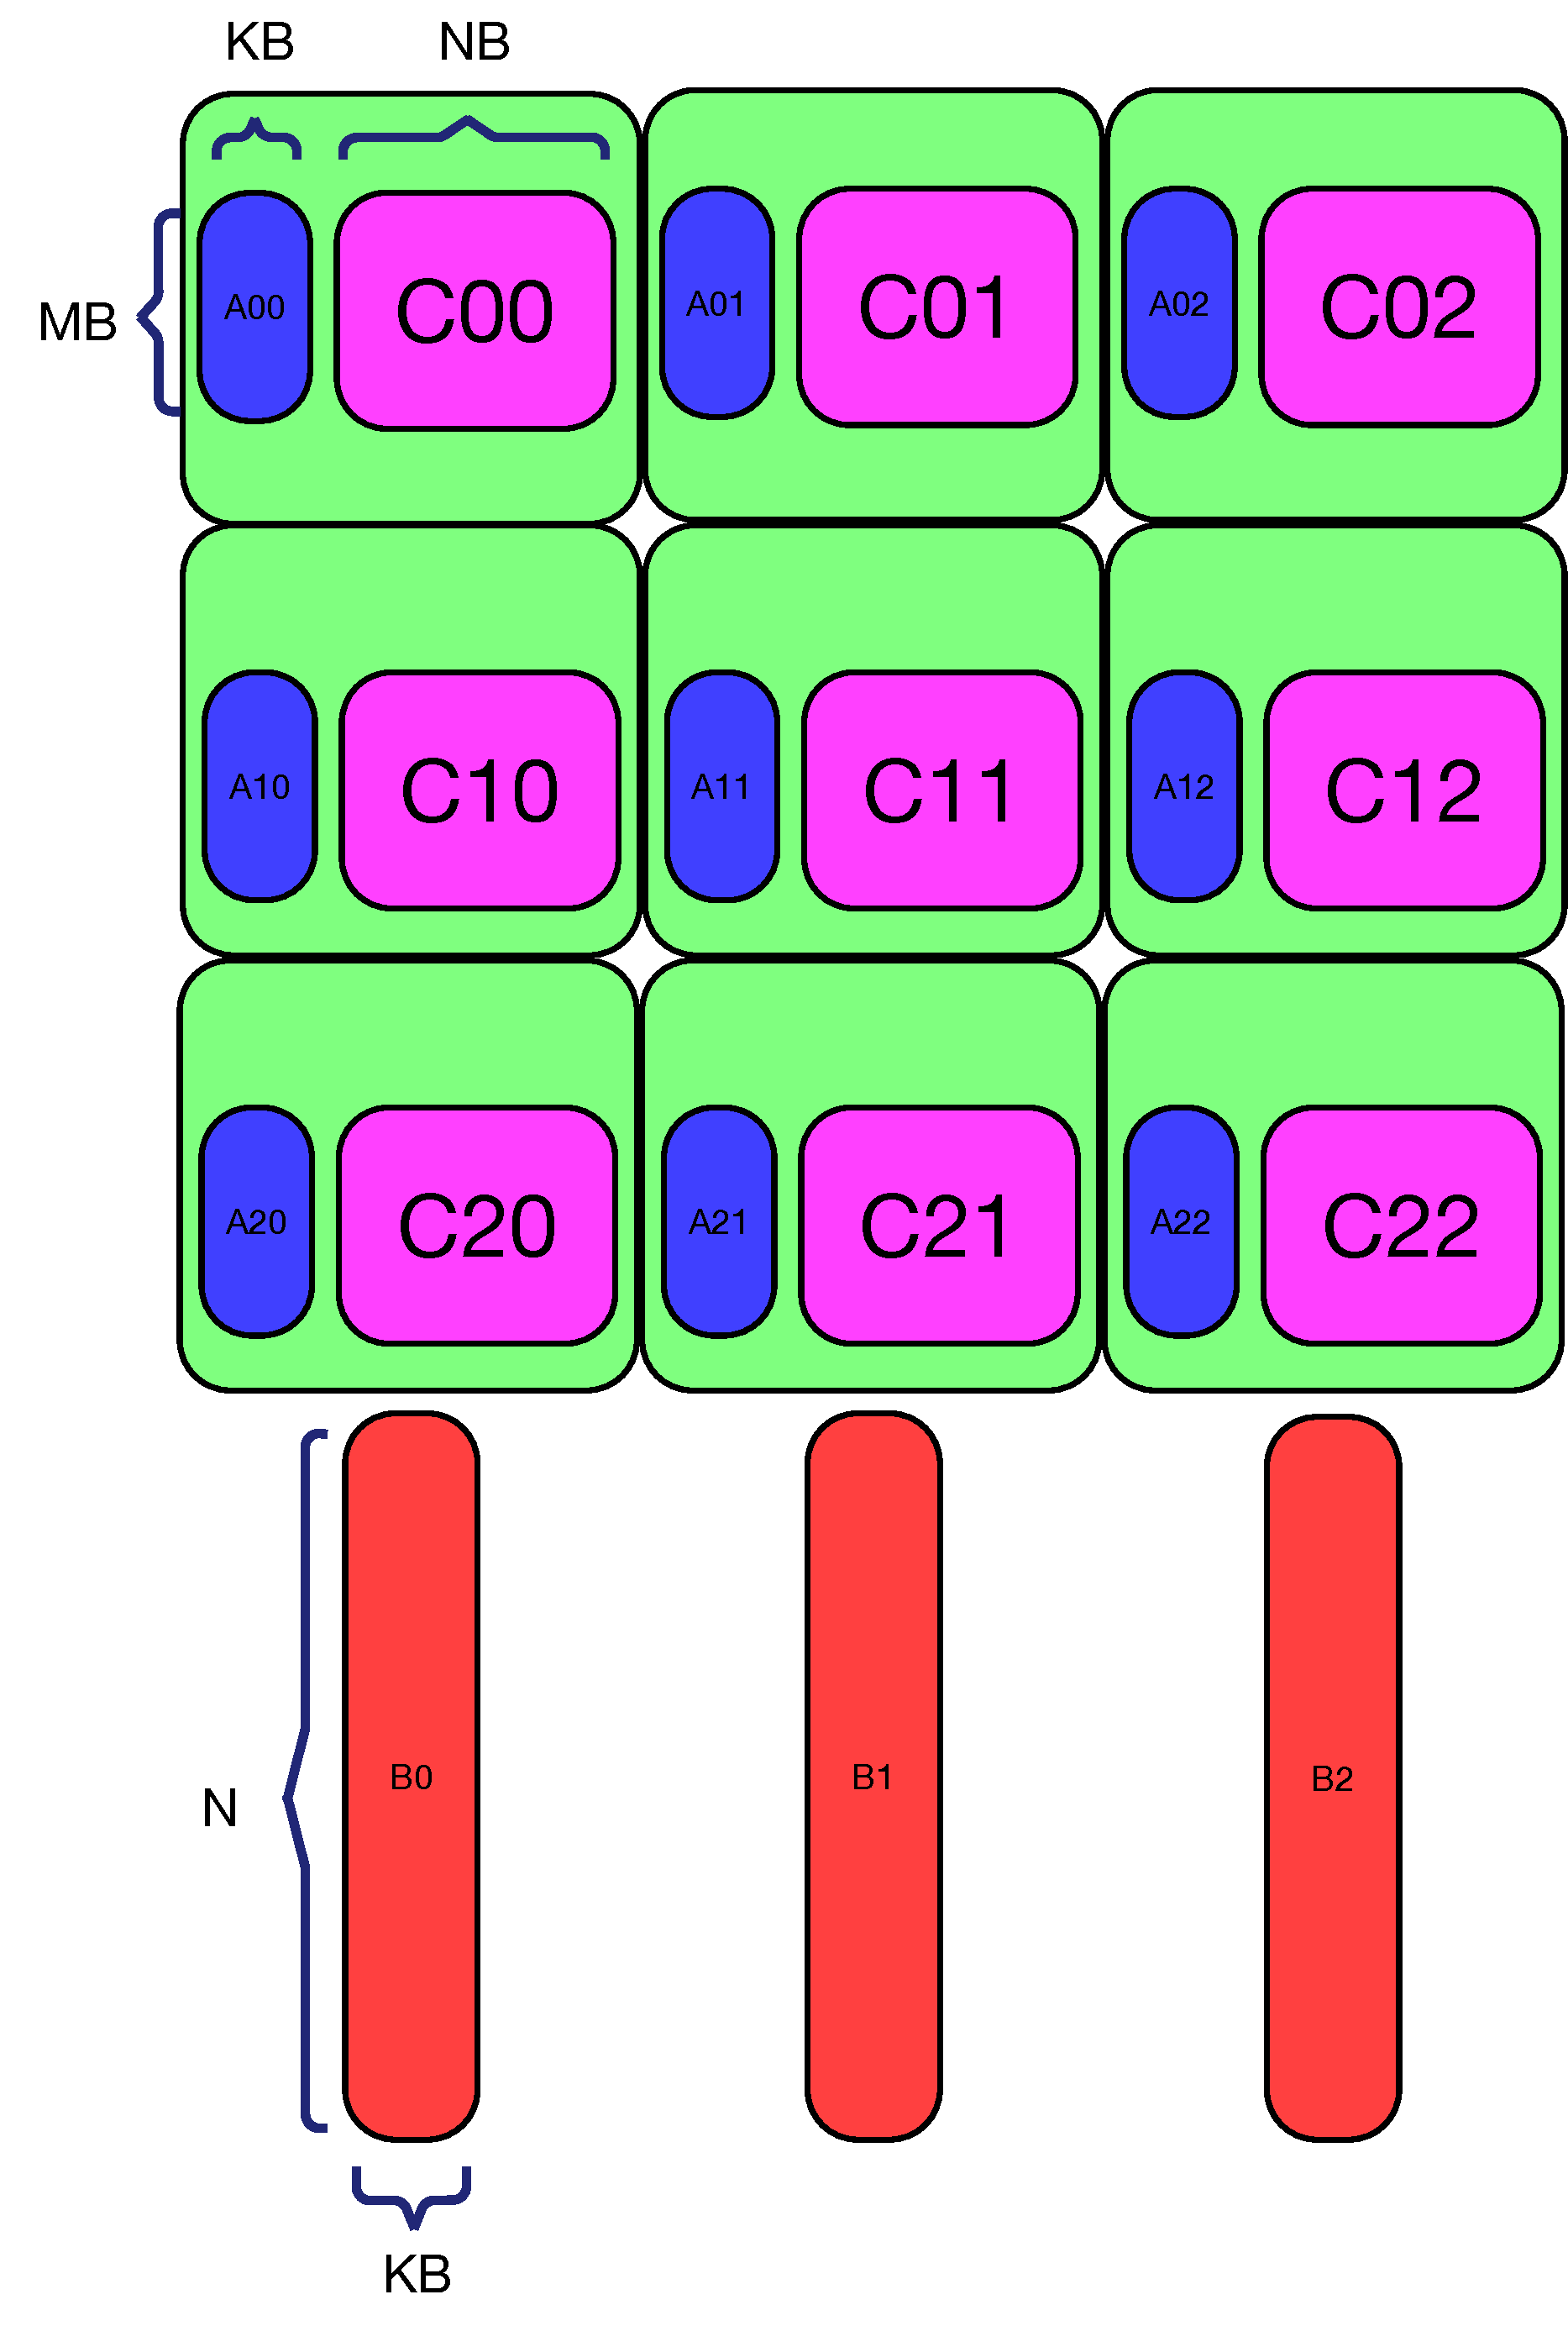
\includegraphics[width=\linewidth]{figures/gemm_A_C_memory_master/1.pdf}
    \caption{Data distribution.}
    \label{fig:gemm_master_1}
  \end{subfigure}
  %
  \begin{subfigure}{0.40\columnwidth}
    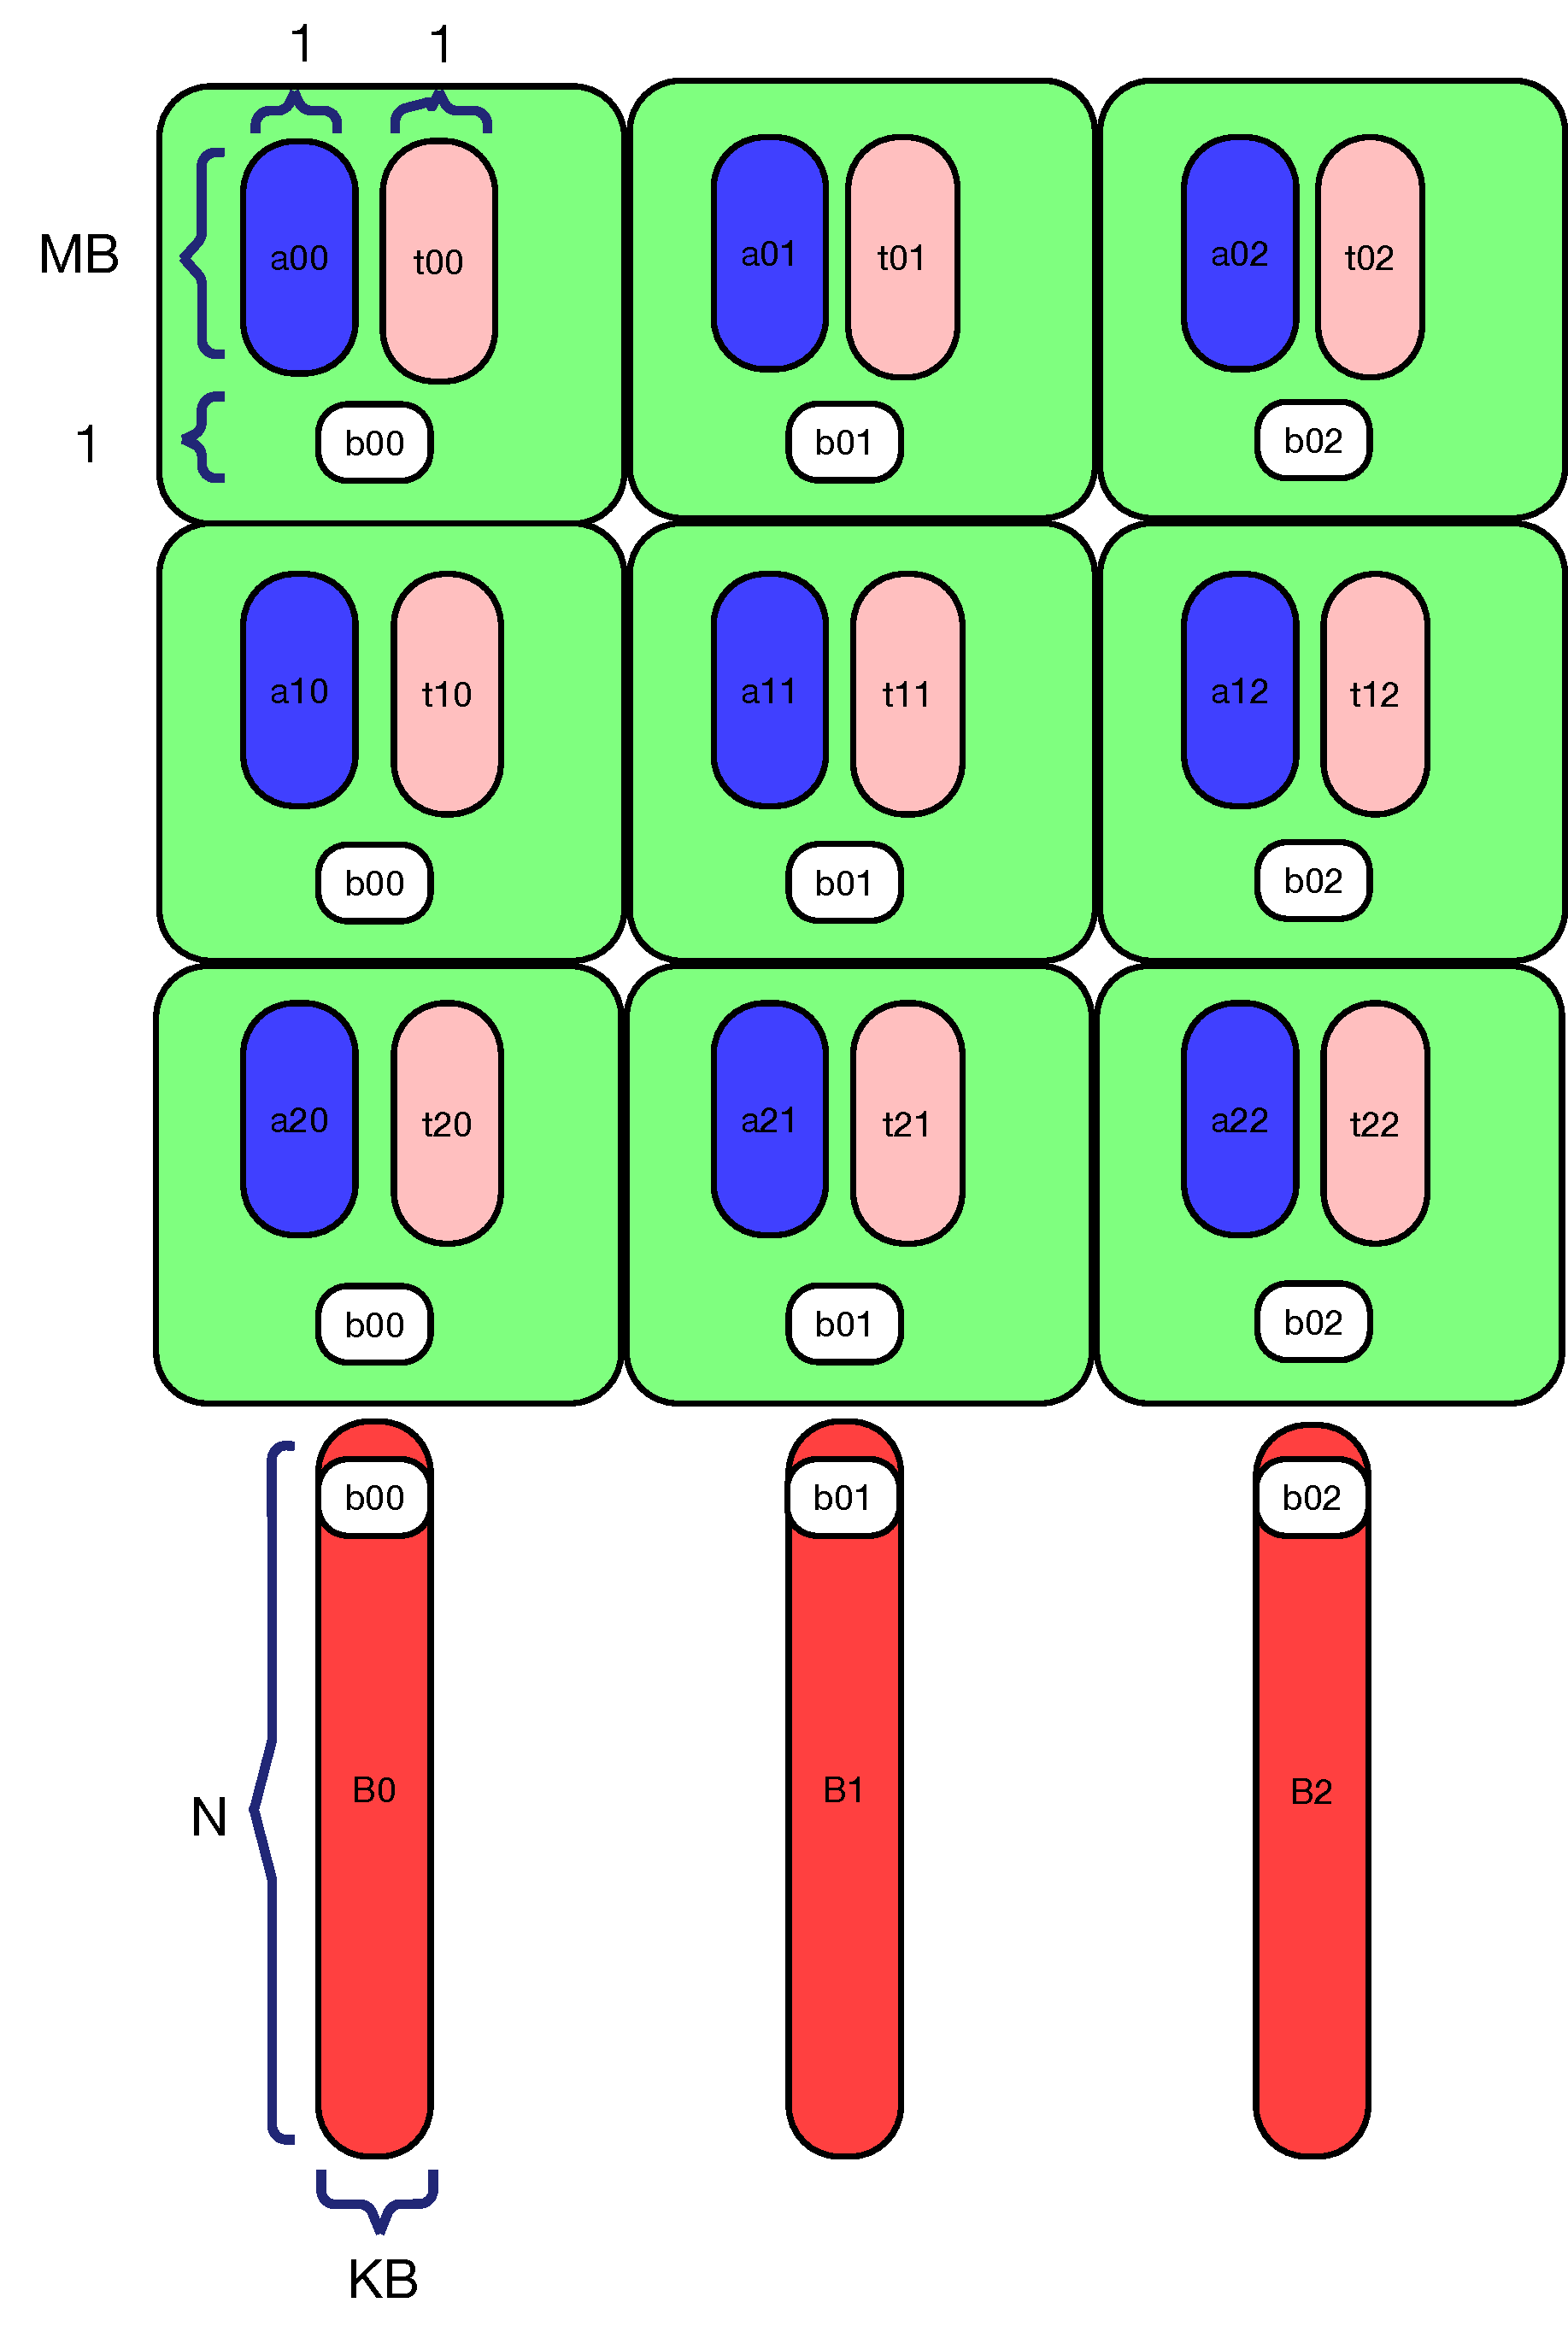
\includegraphics[width=\linewidth]{figures/gemm_A_C_memory_master/2.pdf}
    \caption{The first iteration.}
    \label{fig:gemm_master_2}
  \end{subfigure}
  \caption{\master.}
  \label{fig:gemm_master}
\end{figure}

General Matrix Multiply (\gemm) is a common but widely-used algorithm in linear algebra, machine learning, statistics, and many other domains.
%
It is a level-3 routine in Blas Linear Algebra Subprograms (BLAS)~\cite{blas}, which is compute intensive with $O(N^3)$ flops and $O(N^2)$ data movement, where N is the matrix size.
%
Figure~\ref{fig:gemm_overview} demonstrates an example of ${C}_{M \times N} = A_{M \times K} B_{K \times N}$.
%
Here, a special scenario is considered, called \matmul kernel in weight streaming (WS).
%
It is a variant of \gemm, where one of the inputs ($A$ and $B$) is streamed in from fabric (one feature for \wse).
%
Without loss of generality, let $B$ be streamed in from fabric as weight and $A$ and $C$ be stored in memory as activation, to remove the transpose in the real implementation.
%
Two algorithms are compared, i.e., the method used in the current master (called \master hereinafter) and Scalable Universal Matrix Multiplication Algorithm (\summa~\cite{van1997summa}).